% IEEE Software magazine cut of the UI-as-Policy paper.
% Venue-specific cut derived from the canonical full version.

\documentclass[10pt,journal]{IEEEtran}
\IEEEoverridecommandlockouts

\usepackage{microtype}
\usepackage{url}
\usepackage{xcolor}
\definecolor{CausifyBlue}{HTML}{0369A1}
\usepackage{tikz}
\usepackage{tabularx}
\usepackage{booktabs}
\usepackage[font=small,labelfont=bf]{caption}
\usepackage[colorlinks=true, urlcolor=CausifyBlue, linkcolor=black, citecolor=black]{hyperref}
\usepackage{graphicx}
\usetikzlibrary{arrows.meta, positioning, fit, calc,
                decorations.pathmorphing, decorations.pathreplacing}
\usepackage{lettrine}
\usepackage{enumitem}
\usepackage{xurl}
\usepackage{amsmath}
\usepackage{amssymb}
\usepackage{listings}
\lstset{
  basicstyle=\fontsize{6}{7.5}\selectfont\ttfamily,
  backgroundcolor=\color{gray!10},
  keywordstyle=\color{CausifyBlue},
  morekeywords={const,let,var,function,return,true,false,
                createHmac,randomUUID,update,digest},
  frame=none,
  xleftmargin=0pt, xrightmargin=0pt,
  breaklines=true, breakatwhitespace=false,
  keepspaces=true, columns=flexible
}

\setlength{\emergencystretch}{2em}

\newenvironment{authorbio}[1]{%
  \par\vspace{4pt}%
  \noindent{\small\textbf{#1}}\ \small\ignorespaces%
}{\par\vspace{0pt}}

\AtBeginDocument{\raggedbottom}

% Macros
\newcommand{\system}{the production system}
\newcommand{\uiData}{UI-as-Data}
\newcommand{\uiPolicy}{UI-as-Policy}
\newcommand{\viewas}{view-as}
\newcommand{\code}[1]{{\small\textcolor{CausifyBlue}{\texttt{#1}}}}

\graphicspath{{papers/Causify_Platform_UI_as_Policy/}}

\begin{document}

\title{UI-as-Policy: Unified Permission and Layout System for Multi-Tenant Platforms}

\author{Shayan Ghasemnezhad, Giacinto Paolo (GP) Saggese, Paul Smith, Heanh Sok, and Vedanshubhai Joshi}

\markboth{IEEE Software}{Ghasemnezhad et al.: UI-as-Policy}

\maketitle

% ============================================================

\begin{abstract}
Multi-tenant SaaS products often carry a quiet interface contradiction. Backend policy changes, frontend conditionals lag behind, and users see buttons that return HTTP 403 or modules they cannot use. We present \uiPolicy{}, a production-tested pattern that treats the UI as a policy surface. The backend materializes a tenant- and role-scoped contract; the web tier derives navigation, module visibility, layout, and client-side ability rules from it, while APIs still enforce authorization. Policy changes become reviewed data updates rather than redeploys. The paper defines the representation gap and a Truthful UX invariant for covered surfaces, then describes auditable view-as support workflows. In production, the system manages seven modules, 25+ permission subjects, 150+ layout fields, zero-deployment tenant onboarding, 73--100\% coverage on high-value surfaces, 856 ms P50 full materialization, and 91\% ETag revalidation hits.
\end{abstract}

\begin{IEEEkeywords}
multi-tenant SaaS, authorization, server-driven authorization, UI policy,
impersonation, authorization drift
\end{IEEEkeywords}

% ============================================================

\section{Introduction}

\lettrine[lines=2]{A}{uthorization} bugs are not always spectacular. In multi-tenant SaaS products, they often arrive as small contradictions. The backend denies an action. The frontend still shows it. A restricted tenant sees a module it cannot use. A support engineer cannot tell whether the customer is blocked by policy, configuration, or a stale conditional.

We call this authorization drift. The backend enforces access policy, while the frontend maintains a separate, informal model of what to display. The two models rarely break at once. They drift one branch, one exception, and one tenant-specific rule at a time. The UI then becomes untrustworthy. For users, it feels broken. For operators, it creates avoidable support work. For security and compliance teams, it means the product surface implies access that the backend will not honor.

A concrete example: when onboarding a restricted tenant, a frontend
conditional gating the billing module was not updated alongside the backend
entitlement record. The tenant's sidebar showed the billing link; clicking it
returned HTTP~403. Three support escalations later, a developer traced the
discrepancy to a stale \code{if-block} that was never aligned with the backend
policy record. Under \uiPolicy{}, the sidebar is rendered from the
server-materialized module list; no standalone conditional existed to go stale.

\uiPolicy{} inverts this: instead of the frontend guessing what policy
allows, the backend publishes policy as a structured UI contract and the
frontend renders only what that contract permits. The contract is scoped
by tenant and role, materialized at request time, and treated as a
first-class API response. The same policy inputs that govern authorization
also govern navigation, module visibility, and layout: \uiData{} is the
materialized contract itself, and \uiPolicy{} is the pattern of making that
contract the sole authority for all UI authorization decisions.

Drawing on a deployed production system, this paper makes three contributions:
\begin{itemize}[label=\textbullet, leftmargin=1.2em, topsep=2pt, itemsep=1pt, parsep=0pt, partopsep=0pt]
  \item We characterize the representation gap between backend
    enforcement and frontend rendering, define a Truthful UX invariant,
    and identify three structural conditions sufficient to close it.
    We propose a CI verification procedure that operationalizes the invariant
    as a per-release check.

  \item The production-tested \uiPolicy{} pattern and its core primitive, \uiData{}: a
    server-materialized, tenant- and role-scoped UI contract that drives
    navigation and module composition, paired with a unified ability model
    built server-side and exported read-only to the client.

  \item A \viewas{} design for safe support impersonation: explicit actor
    attribution, HMAC-signed headers, and server-enforced allow-lists that
    preserve auditability without shared admin accounts.
\end{itemize}

Existing authorization frameworks such as OPA, Cedar, Zanzibar~\cite{zanzibar}, and
OpenFGA decide what is permitted but do not prescribe how those decisions
become UI structure. \uiPolicy{} contributes a stack-agnostic discipline that names the invariant,
identifies structural sufficiency conditions, and verifies them in CI, together
with a concrete production-validated realization for products built outside
vendor page-builder platforms.

% ============================================================
\section{Authorization Drift in Multi-Tenant Platforms}

Most multi-tenant applications share the same implicit split: authorization
logic lives in the backend, while the frontend maintains its own parallel set
of conditions for deciding what to display. At small scale, this works. As
the product grows, the two models drift apart and produce a specific,
expensive class of bugs.

We call this the representation gap: the distance between what the
backend would permit and what the UI actually shows. The gap does not require
a bug in the authorization system. It arises simply because the frontend
independently models what to show and, over time, diverges from the backend.

Five requirements define what it means to close the representation gap.
R1, R2, and R4 are universal for multi-tenant SaaS; R3 and R5 apply to
products with support engineering workflows:
\begin{itemize}
  \item[\textbf{R1}] \textbf{No stale gates:} UI elements shown to a user
    must correspond to backend operations the system will actually permit
    for that user's current tenant/role context.

  \item[\textbf{R2}] \textbf{Configuration over redeploy:} Adding a new
    tenant or enabling a feature must not require a code change or
    deployment.

  \item[\textbf{R3}] \textbf{Safe impersonation:} Support engineers must
    adopt a tenant's perspective without sharing credentials or bypassing
    the authorization model.

  \item[\textbf{R4}] \textbf{Defense in depth:} The UI must not be the
    sole barrier to unauthorized access; backend APIs enforce authorization
    independently of what the client renders.

  \item[\textbf{R5}] \textbf{Support at scale:}
    Operators need concurrent session scope and searchable audit logs for
    support workflows at scale. R3 defines the mechanism; R5 defines its
    operational scale properties.
\end{itemize}

Traditional approaches satisfy some of these requirements but not all:
\begin{itemize}[label=\textbullet, leftmargin=1.2em, topsep=2pt, itemsep=1pt, parsep=0pt, partopsep=0pt]
  \item \textbf{RBAC only}: enforces access~(R4) but cannot drive UI
    structure~(R1 unmet) and does not address impersonation or support
    scale~(R3, R5).
  \item \textbf{Feature flags}: support zero-deploy config~(R2) but diverge
    from authorization state over time~(R1 at risk) and do not address
    impersonation or support scale~(R3, R5).
  \item \textbf{OPA/Cedar}: centralize policy and support backend
    enforcement~(R2, R4) but leave the representation gap to the
    application~(R1 partial) and do not prescribe impersonation
    workflows~(R3, R5).
\end{itemize}

OPA/Cedar can in principle drive UI gating, but only when the UI is built
to consume their decisions consistently with backend enforcement; the
representation gap is precisely the work \uiPolicy{} prescribes on top of
such an engine. \uiPolicy{} is designed to address all five requirements.

% ============================================================
\section{System Architecture}

The \uiPolicy{} pattern rests on three implementation-independent
principles: (1)~the backend is the sole authority for UI structure;
(2)~the ability model is built server-side and exported read-only to the
client; and (3)~the frontend derives all rendering decisions by consuming
the contract, never reimplementing permission logic. The contract is a versioned API surface (\code{/v2/me}, with the version
in the path). The production system uses Next.js, DynamoDB, and AWS Lambda;
the three principles are implementation-independent and apply to any
server-rendered or API-driven stack. Figure~\ref{fig:architecture} shows the end-to-end lifecycle.

\begin{figure*}[!t]
  \centering
  \resizebox{!}{0.38\textheight}{%
  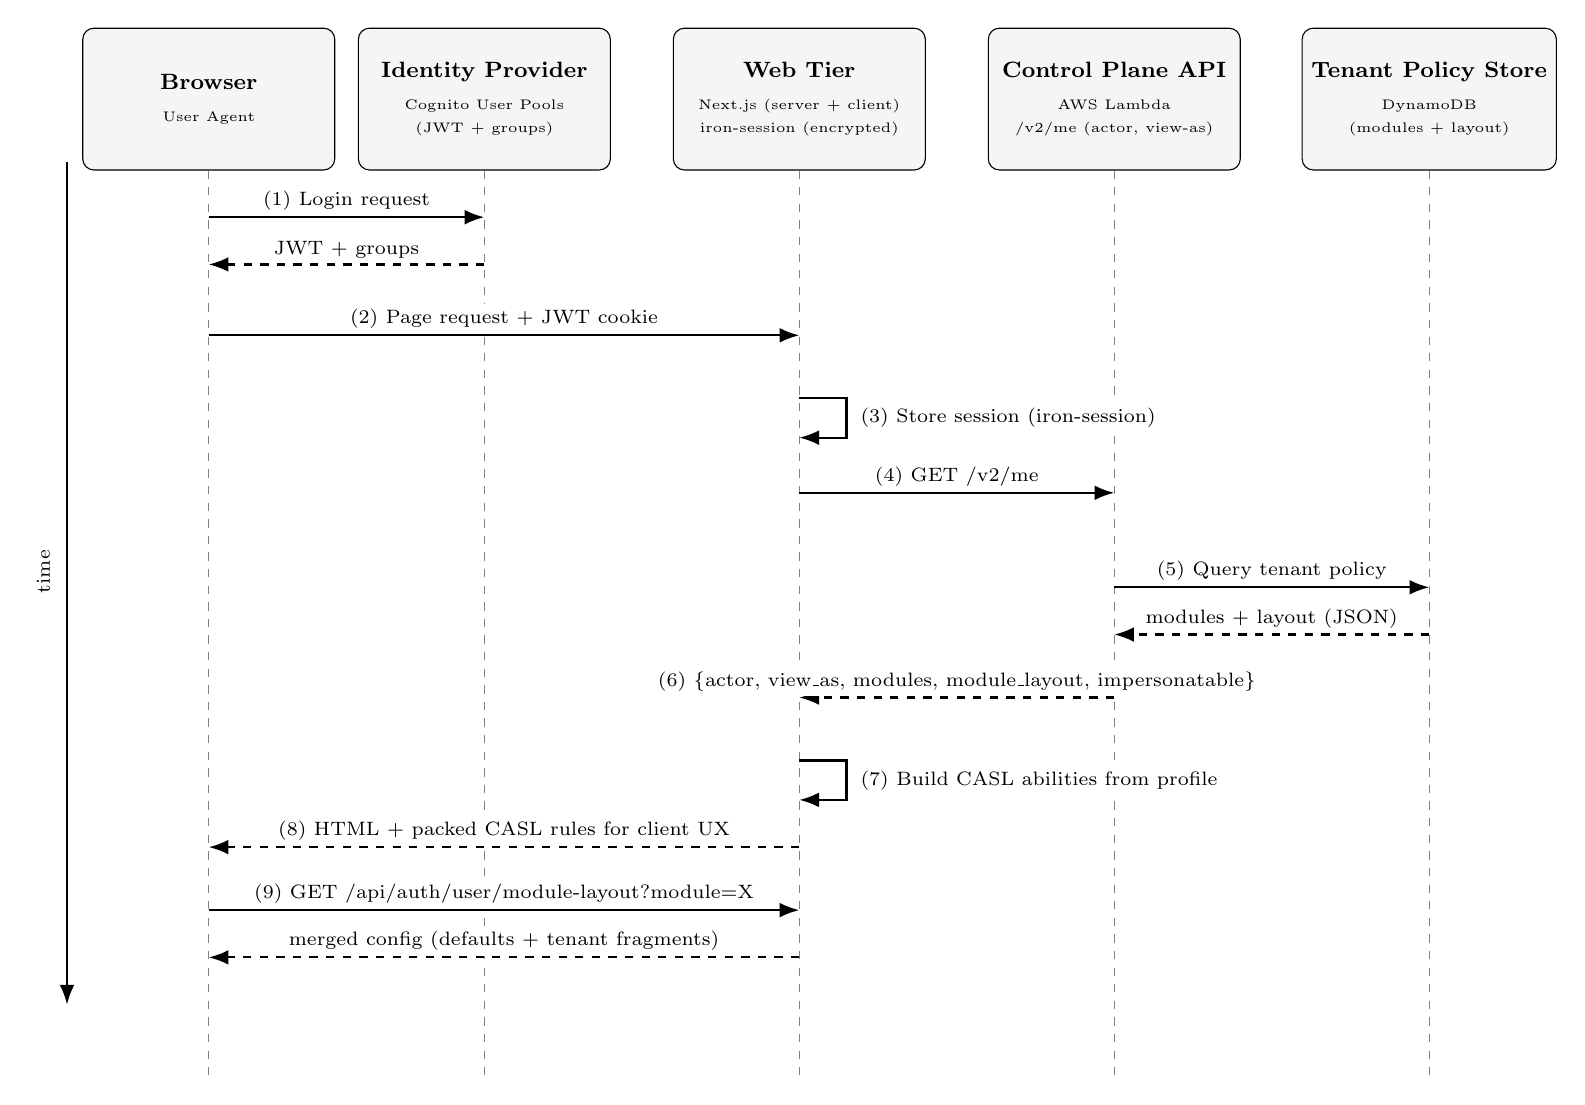
\begin{tikzpicture}[
    actor/.style={draw, rectangle, rounded corners, align=center,
                  minimum width=32mm, minimum height=18mm,
                  font=\footnotesize, fill=gray!8},
    arrow/.style={-{Latex[length=2.5mm]}, thick},
    returnarrow/.style={-{Latex[length=2.5mm]}, thick, dashed},
    lbl/.style={font=\scriptsize, fill=white, inner sep=2pt, align=center},
    lifeline/.style={dashed, gray}
  ]
    \node[actor] (user) at (0,0)    {\textbf{Browser}\\[2pt]\tiny User Agent};
    \node[actor] (idp)  at (3.5,0)  {\textbf{Identity Provider}\\[2pt]\tiny Cognito User Pools\\[-1pt]\tiny (JWT + groups)};
    \node[actor] (web)  at (7.5,0)  {\textbf{Web Tier}\\[2pt]\tiny Next.js (server + client)\\[-1pt]\tiny iron-session (encrypted)};
    \node[actor] (api)  at (11.5,0) {\textbf{Control Plane API}\\[2pt]\tiny AWS Lambda\\[-1pt]\tiny /v2/me (actor, view-as)};
    \node[actor] (ddb)  at (15.5,0) {\textbf{Tenant Policy Store}\\[2pt]\tiny DynamoDB\\[-1pt]\tiny (modules + layout)};

    \draw[lifeline] (user.south) -- ++(0,-11.5);
    \draw[lifeline] (idp.south)  -- ++(0,-11.5);
    \draw[lifeline] (web.south)  -- ++(0,-11.5);
    \draw[lifeline] (api.south)  -- ++(0,-11.5);
    \draw[lifeline] (ddb.south)  -- ++(0,-11.5);

    \draw[arrow]       (0,-1.5) -- node[lbl,above] {(1) Login request} (3.5,-1.5);
    \draw[returnarrow] (3.5,-2.1) -- node[lbl,above] {JWT + groups} (0,-2.1);

    \draw[arrow] (0,-3) -- node[lbl,above] {(2) Page request + JWT cookie} (7.5,-3);

    \draw[arrow] (7.5,-3.8) -- ++(0.6,0) -- ++(0,-0.5) -- ++(-0.6,0);
    \node[lbl,right] at (8.2,-4.05) {(3) Store session (iron-session)};

    \draw[arrow]       (7.5,-5) -- node[lbl,above] {(4) GET /v2/me} (11.5,-5);
    \draw[arrow]       (11.5,-6.2) -- node[lbl,above] {(5) Query tenant policy} (15.5,-6.2);
    \draw[returnarrow] (15.5,-6.8) -- node[lbl,above] {modules + layout (JSON)} (11.5,-6.8);
    \draw[returnarrow] (11.5,-7.6) -- node[lbl,above]
      {(6) \{actor, view\_as, modules, module\_layout, impersonatable\}} (7.5,-7.6);

    \draw[arrow] (7.5,-8.4) -- ++(0.6,0) -- ++(0,-0.5) -- ++(-0.6,0);
    \node[lbl,right] at (8.2,-8.65) {(7) Build CASL abilities from profile};

    \draw[returnarrow] (7.5,-9.5) -- node[lbl,above]
      {(8) HTML + packed CASL rules for client UX} (0,-9.5);

    \draw[arrow]       (0,-10.3) -- node[lbl,above]
      {(9) GET /api/auth/user/module-layout?module=X} (7.5,-10.3);
    \draw[returnarrow] (7.5,-10.9) -- node[lbl,above]
      {merged config (defaults + tenant fragments)} (0,-10.9);

    \draw[-{Latex[length=2.5mm]}, thick] (-1.8,-0.8) -- (-1.8,-11.5);
    \node[font=\scriptsize, rotate=90] at (-2.1,-6.0) {time};
  \end{tikzpicture}%
  }
  \caption{\system{} request lifecycle. The browser authenticates via
  Cognito (1--2). The Web Tier stores the session and fetches the
  materialized UI contract from the Control Plane, which queries DynamoDB
  for tenant policy (3--6). The server builds CASL abilities and returns
  HTML with packed rules (7--8). Module layouts are lazy-loaded on demand
  (9).}
  \label{fig:architecture}
\end{figure*}

The key output is step~6: the \code{/v2/me} response is not merely a
permissions list. It is a structured UI contract containing:
\begin{itemize}
  \item[\textbullet] \textit{actor}: the authenticated identity, immutable across
    the session;
  \item[\textbullet] \textit{view\_as}: the effective tenant/role context, including
    derived modules and layout;
  \item[\textbullet] \textit{modules}: the capability list for navigation composition;
  \item[\textbullet] \textit{module\_layout}: structured UI fragments for the
    navigation bar, sidebar mode, and module defaults;
  \item[\textbullet] \textit{impersonatable}: an explicit allow-list of permissible
    \viewas{} targets for the actor, structured as tenant/role pairs.
\end{itemize}

\noindent A representative \code{/v2/me} response for a two-module tenant:
\noindent\begin{minipage}{\columnwidth}
\begin{lstlisting}
{
  "actor": { "sub": "u123", "email": "e@example.com" },
  "view_as": {
    "tenant_id": "acme",
    "role": "admin",
    "modules": ["horizon", "grid"],
    "module_layout": { "sidebar": "full" } },
  "impersonatable": [
    {"tenant_id":"acme","roles":["member","admin"]},
    {"tenant_id":"globex","roles":["member"]}
  ]
}
\end{lstlisting}
\end{minipage}

The frontend renders navigation from the modules list. It configures
navigation mode, layout visibility, and module components from the
\code{module\_layout} fields. It builds a CASL ability object from the packed rules (step~8) to
hide forbidden UI elements. For policy-gated surfaces, none of this authorization logic is reimplemented on the client.

The platform defines seven independently evolvable production modules.
Each follows an identical structural pattern: a server layout file that enforces
CASL access before rendering, a client component, and dedicated API routes
that inherit the same authorization context. Enabling or disabling a module
for a tenant is a data change in DynamoDB; no deployment is required. The
policy model governing these modules is described next.

% ============================================================
\section{Policy Model and Runtime Composition}

The policy model operates at two levels: coarse-grained module access and
fine-grained feature permissions.

\textbf{Module access} is stored per-tenant, per-role in DynamoDB. Each
record carries a list of enabled modules and a \code{moduleLayout} object
containing structured UI configuration as JSON fragments. The control plane
reads this record during \code{/v2/me} materialization and merges it with
shipped defaults. Malformed or partial configuration is rejected at
ingestion: inconsistent UI composition is treated as a hard error.

\noindent\textbf{Fine-grained permissions} are expressed using CASL~\cite{casl_docs}:
\begin{itemize}[label=\textbullet, leftmargin=1.2em, topsep=2pt, itemsep=1pt, parsep=0pt, partopsep=0pt]
  \item \textbf{Library:} CASL is an isomorphic JavaScript authorization
    library that defines permissions as (action, subject) rules and supports
    serialization between server and client.
  \item \textbf{Scope:} The ability model covers three actions (view, manage,
    and use) across 25+ subjects: seven modules, five generic pages, 16
    feature permissions (\code{feature:export}, \code{feature:admin}, etc.),
    sub-module subjects, and config-derived subjects from \code{moduleLayout}
    paths (for example, \code{module:config:integration:enabled}).
  \item \textbf{Server-side construction:} The ability model is built entirely
    on the server from the materialized \code{/v2/me} profile; the client
    receives it as packed rules and uses it exclusively for UX decisions.
\end{itemize}

Module-specific layout is loaded lazily via \code{/api/auth/user/module-layout}.
This endpoint performs a server-side ability check before serving the
configuration: a module's layout is itself a privileged resource. If the
user cannot view a module, the server will not return its layout even if
the client requests it directly. Tenant fragments are deep-merged over
shipped defaults, so partial overrides are safe. A tenant can override one component without redefining the entire module
configuration.

The architecture scales horizontally: adding a tenant requires no schema
change, no deployment, and no service restart. The per-request cost is
bounded by a single policy store lookup and a CASL rule compilation step,
both O(subjects); the compilation itself is fast and the observed 856\,ms
warm P50 is attributable to JWKS validation and the DynamoDB read overhead. The impersonation mechanism built on this model is
described next.

% ============================================================
\section{Safe Impersonation Without Shared Accounts}\label{sec:impersonation}

Support engineers regularly need to see a tenant's UI exactly as that
tenant's users see it. The usual shortcut is a shared admin account that
bypasses normal access control. It is convenient in the moment and expensive
later: auditing becomes murky, risk concentrates into one credential, and the
paper trail that compliance teams need is gone.

Our \viewas{} feature addresses this problem with three design decisions:
\begin{itemize}[label=\textbullet, leftmargin=1.2em, topsep=2pt, itemsep=2pt, parsep=0pt, partopsep=0pt]
  \item \textbf{Actor attribution is immutable:} The \code{actor} field in
    \code{/v2/me} always reflects the real authenticated identity: the support
    engineer's own account. The \code{view\_as} field represents the effective
    tenant/role being adopted. These are never conflated. Every API call made
    during a view-as session is logged with both identities.

  \item \textbf{Allow-lists are server-enforced:} The control plane computes an
    \code{impersonatable} list from the actor's role and validates the
    \code{X-View-As} header against it before applying any effective context.
    A support engineer cannot impersonate a tenant outside their authorized
    scope. This enforcement lives in the Lambda middleware, not in UI code.

  \item \textbf{Signed effective context:} The web tier signs the requested
    \code{X-View-As} context with HMAC-SHA256. The signature is stored in the
    encrypted server-side session and the browser never sees the key. Each
    activation receives a nonce, and the control plane rejects a header whose
    nonce is missing or revoked. Logout and tenant switches revoke the active
    context immediately; a replayed header also requires a live Cognito token.
\end{itemize}

\noindent\begin{minipage}{\columnwidth}
\begin{lstlisting}
// Simplified server-side signing.
const nonce  = randomUUID()
const viewAs = `tenant=${tid};role=${role};nonce=${nonce}`
const sig    = signWithServerKey(viewAs)
\end{lstlisting}
\end{minipage}

The result is a \viewas{} workflow that is fully auditable, with every
session logged and attributable to the engineer's own identity, and free
of shared credentials or bypass logic.
Multiple support engineers can hold concurrent view-as sessions for different
tenants; each session is independently scoped, signed, and logged, satisfying
R5 at operational scale.

% ============================================================
\section{Evaluation}
\phantomsection\label{sec:eval}

We evaluate \uiPolicy{} along five dimensions: truthfulness~(R1,~R4),
operational leverage~(R2), policy depth, runtime cost, and defense in
depth. The \viewas{} design in Section~\ref{sec:impersonation} addresses R3 and R5.

\noindent\textbf{Threat model.} \uiPolicy{} defends against stale UI gates (addressed
by the Truthful UX invariant below), impersonation abuse (addressed by
Section~\ref{sec:impersonation}), and client-side authorization bypass (addressed by backend
enforcement independent of whatever the client renders).

\noindent\textbf{The policy store is the new critical surface.} Moving policy from
code to DynamoDB shifts the blast radius of a malicious or buggy write from
``one tenant'' to ``the UI contract for every user of that tenant.''
The production system mitigates this with IAM-scoped writes, change review,
and strict JSON parsing at materialization, but the surface remains and
operators must treat policy-store writes with the same scrutiny as code
deploys. Out-of-scope threats are addressed by standard cloud controls and
not covered here.

\noindent\textbf{Open gaps (planned mitigations):}
\begin{itemize}[label=\textbullet, leftmargin=2em, topsep=2pt, itemsep=1pt, parsep=0pt, partopsep=0pt]
  \item Policy takes effect at next page load; planned: push updates via DynamoDB Streams.
  \item JSON schema ungoverned across versions; planned: add JSON Schema validation with CI gate.
\end{itemize}

\noindent\textbf{Mitigations implemented:}
\begin{itemize}[label=\textbullet, leftmargin=2em, topsep=2pt, itemsep=1pt, parsep=0pt, partopsep=0pt]
  \item Browser CASL tampering: backend enforces authorization independently.
  \item \code{X-View-As} header injection: HMAC-SHA256 signing with server-side validation.
  \item Session replay: iron-session encryption and TTL.
  \item Unlicensed module request: \code{can('view',\,module)} server check before serving layout.
  \item Stale DynamoDB policy read: bounded by page-load cadence.
\end{itemize}

\noindent\textbf{Truthful UX invariant.} The system prevents drift through three
structural properties: (i)~navigation is rendered exclusively from
\code{view\_as.modules} in the \code{/v2/me} response; (ii)~module layout
is served only when \code{can('view',\,module)} holds server-side;
(iii)~backend APIs enforce authorization independently of the client.
Properties (i) and (ii) mean covered UI surfaces cannot show module
structure the backend would deny. Both the navigation set and the layout
served derive from the same record that governs backend authorization.
Property (iii) bounds damage if a gap opens despite the
first two.
We automate this as a CI door check: for each (tenant,~role) pair in a
test matrix:
\begin{itemize}[label=\textbullet, leftmargin=1.2em, topsep=3pt, itemsep=1pt, parsep=0pt, partopsep=0pt]
  \item Fetch \code{/v2/me} and extract the licensed module list $M$.
  \item Check module layout fetches: licensed modules return HTTP~200; unlicensed
    modules return HTTP~403.
  \item Check routes: routes in $M$ render; routes outside $M$ return HTTP~403 or
    redirect.
\end{itemize}

\begin{table}[h!]
  \centering
  \caption{Policy adoption and coverage metrics for the production deployment.
  Coverage = fraction of surface components that conditionally render based on
  at least one CASL ability check or module membership test.}
  \label{tab:eval_summary}
  \small
  \begin{tabularx}{\columnwidth}{X r}
    \toprule
    \textbf{Metric} & \textbf{Value} \\
    \midrule
    Modules defined in policy store         & 7 \\
    CASL permission subjects                & 25+ \\
    \code{moduleLayout} config fields       & 150+ \\
    Tenant onboardings requiring deployment & 0 \\
    \midrule
    \textbf{Policy surface coverage:}       & \\
    Navigation items                        & 8/11 (73\%) \\
    Module components                       & 7/7 (100\%) \\
    Configuration tabs                      & 5/6 (83\%) \\
    \midrule
    \multicolumn{2}{l}{\textbf{UI elements hidden for restricted tenant (by module count):}} \\
    Single-module tenant                    & 6/7 (86\%) \\
    Two-module tenant                       & 5/7 (71\%) \\
    \bottomrule
  \end{tabularx}
\end{table}

\noindent\textbf{Operational leverage.} The platform serves more than ten tenants,
each with multiple users across roles (admin, member, and others); Cognito
groups map many-to-one to tenants, so a single group can represent multiple
tenant contexts. Adding a tenant is a data operation: one DynamoDB record,
one Cognito group assignment. No code change, no deployment. The 150+
\code{moduleLayout} fields take effect at the next page load.

\noindent\textbf{Policy depth.} We define policy coverage as the fraction of
components in a surface that conditionally render based on at least one
CASL ability check or module membership test. Layout and navigation
components decide what is rendered; most leaf components inherit those
decisions transitively through their parents, which is typical of React
codebases. High-value surfaces (navigation, module components,
configuration) carry 73--100\% policy coverage. For example,
a single-module tenant sees 86\% of the full-featured module list suppressed;
the absolute component counts are omitted here because the meaningful outcome
metric is zero-deployment onboarding, not component percentages.

\noindent\textbf{Drift reduction.} Before adoption, permission and navigation
mismatches generated recurring support escalations requiring developer
investigation. Since adoption, we have observed no drift incidents against
policy-gated surfaces. The 27\% of navigation items not under coverage are
generic components intentionally shared across all roles and tenants.

\noindent\textbf{Runtime cost.} Table~\ref{tab:runtime} reports CloudWatch warm-path
latency for the full materialization of \code{/v2/me} at 512\,MB. The 856\,ms
warm P50 covers the complete path: JWKS validation, tenant and role reads,
JSON fragment assembly, and CASL compilation. This cost is paid once per
session: ETag-conditional revalidations dominate steady-state traffic at a
91\% hit rate, with a 304 response P50 of 68\,ms and median user-visible
latency of 75\,ms.

\begin{table}[h!]
  \centering
  \caption{Controller Lambda full-materialization latency
  (1{,}368 production observations; March--April~2026; 512\,MB configuration).}
  \label{tab:runtime}
  \small
  \begin{tabularx}{\columnwidth}{X r}
    \toprule
    \textbf{Metric} & \textbf{512\,MB (ms)} \\
    \midrule
    P50      & 856     \\
    P75      & 938     \\
    P90      & 1{,}038 \\
    P95      & 1{,}112 \\
    P99      & 1{,}176 \\
    \bottomrule
  \end{tabularx}
\end{table}

\noindent\textbf{Defense in depth.} Six enforcement layers protect every request between
the browser and the data plane. No single layer is the sole barrier; a failure
in any one does not compromise the remaining five. This satisfies R4: the
control plane enforces authorization regardless of what the client renders, so
a misconfigured CASL rule or tampered browser state cannot produce a permitted
backend response.
\begin{itemize}[label=\textbullet, leftmargin=1.2em, topsep=2pt, itemsep=1pt, parsep=0pt, partopsep=0pt]
  \item Edge middleware enforces path validation, injects security headers, and redirects unauthenticated sessions.
  \item Server components redirect to login when \code{getSession()} finds no valid session.
  \item CASL abilities are built server-side from \code{/v2/me} and exported to the client for UX rendering only.
  \item Module gating requires a passing \code{can('view',\,module)} check before the server returns layout config.
  \item View-as requests are signed with HMAC-SHA256 on \code{X-View-As}; the secret never leaves the server.
  \item The control plane Lambda validates the JWT, allow-list membership, and schema prefix for the per-tenant DB namespace.
\end{itemize}

\noindent\textbf{What this evaluation does and does not show.}
The evaluation is correctness-based: UI-backend alignment is guaranteed by
construction for covered surfaces (73--100\% policy coverage); the remaining
gap corresponds to legacy components not yet migrated. Longitudinal drift
quantification and full CI door-checks against a tenant matrix remain as
planned extensions.

% ============================================================
\section{Related Work}

\noindent\textbf{RBAC, ABAC, and policy formalisms.}
Role-based access control (RBAC) formalizes role-to-permission assignment~\cite{sandhu_rbac}.
ABAC formalizes
authorization decisions based on attributes rather than static
roles~\cite{nist_abac}, and XACML standardizes the PEP/PDP separation
that underlies most modern authorization systems~\cite{xacml}.
\uiPolicy{} extends these frameworks by consuming any ability model and
making the covered UI surfaces reflect it.

\noindent\textbf{Feature toggles.} Feature flags separate release from
deployment~\cite{fowler_feature_toggles}, but can diverge from authorization
state, recreating the representation gap at a different level; \uiPolicy{}
extends this idea by scoping configuration per tenant/role and validating it
against the same ability model.

\noindent\textbf{Policy engines.} OPA~\cite{opa_docs},
Cedar~\cite{cedar_docs,aws_verified_permissions}, and OpenFGA~\cite{openfga_docs}
centralize authorization logic; we build on these by prescribing how their
decisions are faithfully reflected in UI structure, a problem these engines
leave to the application.

\noindent\textbf{Impersonation and operational risk.} OWASP classifies account
impersonation as a key security risk~\cite{owasp_impersonation}; our \viewas{}
design extends standard recommendations with immutable actor attribution,
server-enforced allow-lists, and HMAC-signed headers.

\noindent\textbf{Frontend authorization patterns.} OWASP classifies broken
access control as the top web security risk~\cite{owasp_broken_access}.
Client-side approaches (role-based rendering, route guards) operate exclusively
on the client and are vulnerable to drift; \uiPolicy{} extends this practice
by making the server the primary authority for both security enforcement and
UI structure.

\noindent\textbf{Permission-driven UI in enterprise platforms.} Enterprise
platforms have shipped permission-coupled UI for years: Salesforce Lightning
binds page composition to permission sets~\cite{salesforce_lightning};
ServiceNow's UI Policies modify form behavior server-side based on
roles~\cite{servicenow_ui_policy}. \uiPolicy{} differs in scope: those
systems realize the pattern inside a vendor page-builder product, while
\uiPolicy{} presents it as an exportable architectural discipline (the
Truthful UX invariant, structural sufficiency conditions, CI verification)
for products built outside such platforms.

\noindent\textbf{Server-Driven UI.} SDUI architectures~\cite{airbnb_sdui}
return layout from the server, improving flexibility without deployments, but
do not address authorization correctness. \uiPolicy{} builds on SDUI by
coupling the layout contract to the authorization model: the same inputs that
determine permissions determine structure.

% ============================================================
\section{Conclusion}\label{sec:conclusion}

\uiPolicy{} makes authorization visible for policy-gated surfaces: if a user
can reach it in the UI, the backend has licensed it. As an experience report from a deployed
production system, this paper demonstrates that materializing a
server-authoritative UI contract per-tenant and per-role, and deriving both
UX and authorization from a single unified ability model, reduces the
representation gap through architectural discipline, turns tenant variability into
a data operation, and gives support engineers a safe way to see what their
tenants see without shared credentials.

Three open technical gaps (HMAC scope, page-load policy latency, and
ungoverned JSON schema) are enumerated with planned mitigations in
Section~\ref{sec:eval}. The remaining work is longitudinal: drift incident
quantification across the adoption boundary and continuous CI door-checks
against a full tenant matrix.

% IEEE Software requires three actionable insights
\noindent\textbf{Takeaways for Practitioners}
\begin{itemize}[label=\textbullet, leftmargin=1.2em, topsep=2pt, itemsep=1pt, parsep=0pt, partopsep=0pt]
  \item \textbf{Treat the UI as a security boundary, not a presentation
    layer:} If the frontend independently models permissions, drift is
    inevitable. Derive UI structure from the same inputs that decide
    authorization.
  \item \textbf{Store tenant variability as data, not as code branches:}
    Per-tenant feature sets and layout fragments belong in a policy
    store, not in \code{if (tenant === 'acme')} conditionals. The
    payoff is zero-deployment onboarding.
  \item \textbf{Separate actor from effective context for safe
    impersonation:} Never share admin credentials for support. An
    immutable actor identity plus a server-validated allow-list of
    \viewas{} targets preserves the audit trail.
\end{itemize}

% Keep this reference set at or below the IEEE Software limit.
\bibliographystyle{IEEEtran}
\bibliography{references}

\section*{About the Authors}

\begin{authorbio}{Shayan Ghasemnezhad}
is Infrastructure and DevOps Lead at Causify AI, Turin, Italy. His research interests include platform engineering and cloud solutions architecture, production AI/ML systems, and secure, reliable infrastructure operations. Ghasemnezhad received his Bachelor's degree in Digital Management from Ca' Foscari University of Venice. Contact him at shayan@causify.ai.
\end{authorbio}

\begin{authorbio}{Giacinto Paolo (GP) Saggese}
is Co-founder and CTO at Causify AI, Potomac, Maryland, USA. His research interests include machine learning, fintech, and the commercialization of research. Saggese received his Ph.D. degree in Electrical and Computer Engineering from the University of Illinois Urbana-Champaign. He is an Adjunct Professor at the University of Maryland, College Park. Contact him at gp@causify.ai.
\end{authorbio}

\begin{authorbio}{Paul Smith}
is Co-founder and Chief Scientist at Causify AI, Cary, North Carolina, USA. His research interests include causal inference, Bayesian modeling, and time-series prediction. Smith received his Ph.D. degree in Mathematics from UCLA. Contact him at paul@causify.ai.
\end{authorbio}

\begin{authorbio}{Heanh Sok}
is Software Engineer at Causify AI, College Park, Maryland, USA. His research interests include big data systems, distributed systems, and AI/ML engineering and operations. Sok received his Master's degree in Data Science from the University of Maryland, College Park. Contact him at h.sok@causify.ai.
\end{authorbio}

\begin{authorbio}{Vedanshubhai Joshi}
is Software Engineer at Causify AI, Indiana, USA. His research interests include platform infrastructure, multi-tenant API design, and data engineering pipelines. Joshi received his Master's degree in Computer Science from Purdue University. Contact him at v.joshi@causify.ai.
\end{authorbio}
\end{document}
